\documentclass[handout]{ximera}

\title{Video Set Introduction}

\begin{document}

\begin{abstract}
\end{abstract}

%Vid Set 3: Graphing Derivatives

\maketitle


\begin{javascript}
  nameCheck = function(a,b) {
    return a.toLowerCase() != b.toLowerCase();
  };
\end{javascript}

Before watching the videos, think about and answer these questions to the best of your ability. Your answer will always be recorded as correct, regardless of your answer choice.

The graph of the function $g$ is shown below.

\begin{image}
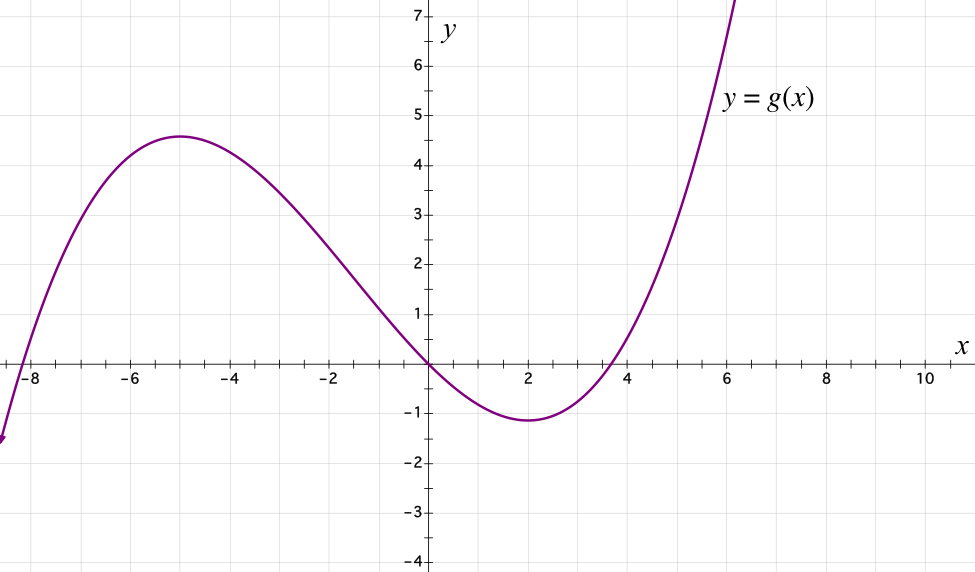
\includegraphics{Picture1.png}
\end{image}

\begin{problem}
Approximate the value of $g'(-1)$
$\answer[format=string,validator=nameCheck]{}$.
\end{problem}


\begin{problem}
For how many values of $x$ in the interval $[-8, 6]$ does $g'(x)=0$? (Just enter the number of values.)
$\answer[format=string,validator=nameCheck]{}$.
\end{problem}


\begin{problem}
Which of the following values is the largest?

\begin{multipleChoice}
\choice[correct]{$g'(-7)$}
\choice[correct]{$\dfrac{g(-5)-g(-7)}{2}$}
\choice[correct]{1}
\choice[correct]{$g'(2)$}
\end{multipleChoice}

\end{problem}

\end{document}
